% Options for packages loaded elsewhere
\PassOptionsToPackage{unicode}{hyperref}
\PassOptionsToPackage{hyphens}{url}
%
\documentclass[
  english,
  man]{apa7}
\usepackage{amsmath,amssymb}
\usepackage{lmodern}
\usepackage{ifxetex,ifluatex}
\ifnum 0\ifxetex 1\fi\ifluatex 1\fi=0 % if pdftex
  \usepackage[T1]{fontenc}
  \usepackage[utf8]{inputenc}
  \usepackage{textcomp} % provide euro and other symbols
\else % if luatex or xetex
  \usepackage{unicode-math}
  \defaultfontfeatures{Scale=MatchLowercase}
  \defaultfontfeatures[\rmfamily]{Ligatures=TeX,Scale=1}
\fi
% Use upquote if available, for straight quotes in verbatim environments
\IfFileExists{upquote.sty}{\usepackage{upquote}}{}
\IfFileExists{microtype.sty}{% use microtype if available
  \usepackage[]{microtype}
  \UseMicrotypeSet[protrusion]{basicmath} % disable protrusion for tt fonts
}{}
\makeatletter
\@ifundefined{KOMAClassName}{% if non-KOMA class
  \IfFileExists{parskip.sty}{%
    \usepackage{parskip}
  }{% else
    \setlength{\parindent}{0pt}
    \setlength{\parskip}{6pt plus 2pt minus 1pt}}
}{% if KOMA class
  \KOMAoptions{parskip=half}}
\makeatother
\usepackage{xcolor}
\IfFileExists{xurl.sty}{\usepackage{xurl}}{} % add URL line breaks if available
\IfFileExists{bookmark.sty}{\usepackage{bookmark}}{\usepackage{hyperref}}
\hypersetup{
  pdftitle={What determines the similarity of braille letters? A matrix of perceived letter similarity in braille by blind individuals},
  pdfauthor={Ana Baciero1,2, Pablo Gomez3, Jon Andoni Duñabeitia1,4, \& Manuel Perea1,5},
  pdflang={en-EN},
  pdfkeywords={keywords},
  hidelinks,
  pdfcreator={LaTeX via pandoc}}
\urlstyle{same} % disable monospaced font for URLs
\usepackage{graphicx}
\makeatletter
\def\maxwidth{\ifdim\Gin@nat@width>\linewidth\linewidth\else\Gin@nat@width\fi}
\def\maxheight{\ifdim\Gin@nat@height>\textheight\textheight\else\Gin@nat@height\fi}
\makeatother
% Scale images if necessary, so that they will not overflow the page
% margins by default, and it is still possible to overwrite the defaults
% using explicit options in \includegraphics[width, height, ...]{}
\setkeys{Gin}{width=\maxwidth,height=\maxheight,keepaspectratio}
% Set default figure placement to htbp
\makeatletter
\def\fps@figure{htbp}
\makeatother
\setlength{\emergencystretch}{3em} % prevent overfull lines
\providecommand{\tightlist}{%
  \setlength{\itemsep}{0pt}\setlength{\parskip}{0pt}}
\setcounter{secnumdepth}{-\maxdimen} % remove section numbering
% Make \paragraph and \subparagraph free-standing
\ifx\paragraph\undefined\else
  \let\oldparagraph\paragraph
  \renewcommand{\paragraph}[1]{\oldparagraph{#1}\mbox{}}
\fi
\ifx\subparagraph\undefined\else
  \let\oldsubparagraph\subparagraph
  \renewcommand{\subparagraph}[1]{\oldsubparagraph{#1}\mbox{}}
\fi
% Manuscript styling
\usepackage{upgreek}
\captionsetup{font=singlespacing,justification=justified}

% Table formatting
\usepackage{longtable}
\usepackage{lscape}
% \usepackage[counterclockwise]{rotating}   % Landscape page setup for large tables
\usepackage{multirow}		% Table styling
\usepackage{tabularx}		% Control Column width
\usepackage[flushleft]{threeparttable}	% Allows for three part tables with a specified notes section
\usepackage{threeparttablex}            % Lets threeparttable work with longtable

% Create new environments so endfloat can handle them
% \newenvironment{ltable}
%   {\begin{landscape}\centering\begin{threeparttable}}
%   {\end{threeparttable}\end{landscape}}
\newenvironment{lltable}{\begin{landscape}\centering\begin{ThreePartTable}}{\end{ThreePartTable}\end{landscape}}

% Enables adjusting longtable caption width to table width
% Solution found at http://golatex.de/longtable-mit-caption-so-breit-wie-die-tabelle-t15767.html
\makeatletter
\newcommand\LastLTentrywidth{1em}
\newlength\longtablewidth
\setlength{\longtablewidth}{1in}
\newcommand{\getlongtablewidth}{\begingroup \ifcsname LT@\roman{LT@tables}\endcsname \global\longtablewidth=0pt \renewcommand{\LT@entry}[2]{\global\advance\longtablewidth by ##2\relax\gdef\LastLTentrywidth{##2}}\@nameuse{LT@\roman{LT@tables}} \fi \endgroup}

% \setlength{\parindent}{0.5in}
% \setlength{\parskip}{0pt plus 0pt minus 0pt}

% \usepackage{etoolbox}
\makeatletter
\patchcmd{\HyOrg@maketitle}
  {\section{\normalfont\normalsize\abstractname}}
  {\section*{\normalfont\normalsize\abstractname}}
  {}{\typeout{Failed to patch abstract.}}
\patchcmd{\HyOrg@maketitle}
  {\section{\protect\normalfont{\@title}}}
  {\section*{\protect\normalfont{\@title}}}
  {}{\typeout{Failed to patch title.}}
\makeatother
\shorttitle{Braille letter similarity}
\keywords{keywords\newline\indent Word count: X}
\DeclareDelayedFloatFlavor{ThreePartTable}{table}
\DeclareDelayedFloatFlavor{lltable}{table}
\DeclareDelayedFloatFlavor*{longtable}{table}
\makeatletter
\renewcommand{\efloat@iwrite}[1]{\immediate\expandafter\protected@write\csname efloat@post#1\endcsname{}}
\makeatother
\usepackage{lineno}

\linenumbers
\usepackage{csquotes}
\usepackage{braille}
\usepackage{color}
\ifxetex
  % Load polyglossia as late as possible: uses bidi with RTL langages (e.g. Hebrew, Arabic)
  \usepackage{polyglossia}
  \setmainlanguage[]{english}
\else
  \usepackage[main=english]{babel}
% get rid of language-specific shorthands (see #6817):
\let\LanguageShortHands\languageshorthands
\def\languageshorthands#1{}
\fi
\ifluatex
  \usepackage{selnolig}  % disable illegal ligatures
\fi
\newlength{\cslhangindent}
\setlength{\cslhangindent}{1.5em}
\newlength{\csllabelwidth}
\setlength{\csllabelwidth}{3em}
\newenvironment{CSLReferences}[2] % #1 hanging-ident, #2 entry spacing
 {% don't indent paragraphs
  \setlength{\parindent}{0pt}
  % turn on hanging indent if param 1 is 1
  \ifodd #1 \everypar{\setlength{\hangindent}{\cslhangindent}}\ignorespaces\fi
  % set entry spacing
  \ifnum #2 > 0
  \setlength{\parskip}{#2\baselineskip}
  \fi
 }%
 {}
\usepackage{calc}
\newcommand{\CSLBlock}[1]{#1\hfill\break}
\newcommand{\CSLLeftMargin}[1]{\parbox[t]{\csllabelwidth}{#1}}
\newcommand{\CSLRightInline}[1]{\parbox[t]{\linewidth - \csllabelwidth}{#1}\break}
\newcommand{\CSLIndent}[1]{\hspace{\cslhangindent}#1}

\title{What determines the similarity of braille letters? A matrix of perceived letter similarity in braille by blind individuals}
\author{Ana Baciero\textsuperscript{1,2}, Pablo Gomez\textsuperscript{3}, Jon Andoni Duñabeitia\textsuperscript{1,4}, \& Manuel Perea\textsuperscript{1,5}}
\date{}


\authornote{

Add complete departmental affiliations for each author here. Each new line herein must be indented, like this line.

Enter author note here.

The authors made the following contributions. Ana Baciero: e.g.,, Conceptualization, Design, Data preparation and analyses, Writing - Original Draft Preparation, Writing - Review \& Editing); Pablo Gomez: XXXX; Jon Andoni Duñabeitia: XXXX; Manuel Perea: XXXX.

Correspondence concerning this article should be addressed to Ana Baciero, Santa Cruz de Marcenado, 27. 28015, Madrid,Spain. E-mail: \href{mailto:abaciero@nebrija.es}{\nolinkurl{abaciero@nebrija.es}}

}

\affiliation{\vspace{0.5cm}\textsuperscript{1} Universidad Antonio de Nebrija\\\textsuperscript{2} DePaul University\\\textsuperscript{3} California State University San Bernardino, Palm Desert Campus\\\textsuperscript{4} The Arctic University of Norway\\\textsuperscript{5} Universitat de València}

\abstract{
One or two sentences providing a \textbf{basic introduction} to the field, comprehensible to a scientist in any discipline.

Two to three sentences of \textbf{more detailed background}, comprehensible to scientists in related disciplines.

One sentence clearly stating the \textbf{general problem} being addressed by this particular study.

One sentence summarizing the main result (with the words ``\textbf{here we show}'' or their equivalent).

Two or three sentences explaining what the \textbf{main result} reveals in direct comparison to what was thought to be the case previously, or how the main result adds to previous knowledge.

One or two sentences to put the results into a more \textbf{general context}.

Two or three sentences to provide a \textbf{broader perspective}, readily comprehensible to a scientist in any discipline.
}



\begin{document}
\maketitle

\hypertarget{introduction}{%
\section{Introduction}\label{introduction}}

TEXT INTRO

26 basic letters of the Latin alphabet

\hypertarget{experiment-1-depaul}{%
\section{Experiment 1: DePaul}\label{experiment-1-depaul}}

\hypertarget{method}{%
\subsection{Method}\label{method}}

Only passive

\hypertarget{participants}{%
\subsubsection{Participants}\label{participants}}

86 undergraduate students at DePaul University who did not know how to read braille were recruited through the subject pool system. All of them gave informed consent before their participation and earned one course-credit for taking part in the study. With this sample size, we wanted to ensure each pair of different letters was observed a minimum of 15 times (considering pairs containing the same two different letters in the opposite order as being different pairs {[}e.g., \braille{l} \braille{f} different from \braille{f} \braille{l}{]}, and taking into account that some trials may be lost in data cleaning).

\hypertarget{materials}{%
\subsubsection{Materials}\label{materials}}

The study used all possible 2-letter combinations: 676 pairs. Out of those pairs, 26 were the same two letters (e.g., \braille{f} \braille{f}), and 650 two different letters (e.g., \braille{f} \braille{t}). Thus, five different lists of pairs were created in which 130 were same pairs (i.e., formed by the same two letters), and 130 were different pairs (i.e., formed by two different letters). Each participant perceived 266 trials, where 6 were practice and 260 were target trials; the order of presentation was randomized for each participant.

\textbf{3 PARTICIPANTS (87-89) ONLY 210!}

\hypertarget{procedure}{%
\subsubsection{Procedure}\label{procedure}}

The experiment took place individually in a quiet room. Participants used the moving version of TouchScope. Hence, participants did not move their fingers to perceive the stimuli. They were instructed to place their index fingertip on the start position to let the braille display slide against it. The braille display moved for 5 cm at 38.9 mm/s (35.9 mm/rev x 65 rpm / 60). This speed was chosen considering previous studies on passive touch (see Vega-Bermudez et al., 1991), as well as our own experience testing it. After moving said distance, the display stopped until participants responded and reset its position during the one-second ITI. This experiment also took around 30 minutes to complete.

\hypertarget{data-analysis}{%
\subsubsection{Data analysis}\label{data-analysis}}

\hypertarget{results}{%
\subsection{Results}\label{results}}

\begin{verbatim}
## [1] 14
\end{verbatim}

\begin{verbatim}
## Bayes factor analysis
## --------------
## [1] Alt., r=0.707 : 2955488 ±0%
## 
## Against denominator:
##   Null, mu = 0 
## ---
## Bayes factor type: BFoneSample, JZS
\end{verbatim}

\begin{verbatim}
## Bayes factor analysis
## --------------
## [1] Alt., r=0.707 : 0.1300824 ±0%
## 
## Against denominator:
##   Null, mu = 0 
## ---
## Bayes factor type: BFoneSample, JZS
\end{verbatim}

\begin{tabular}{l|r|r|r|r|r|r|r|r|r|r|r|r|r|r|r|r|r|r|r|r|r|r|r|r|r|r}
\hline
  & a & b & c & d & e & f & g & h & i & j & k & l & m & n & o & p & q & r & s & t & u & v & w & x & y & z\\
\hline
a & NA & 0.979 & 0.948 & 0.992 & 0.992 & 0.930 & 0.944 & 0.906 & 0.915 & 0.954 & 1.008 & 0.946 & 0.940 & 0.935 & 0.924 & 0.863 & 0.967 & 0.922 & 0.988 & 0.936 & 0.928 & 0.921 & 1.020 & 0.980 & 0.941 & 0.903\\
\hline
b & 0.979 & NA & 0.993 & 1.026 & 0.988 & 0.990 & 0.990 & 0.969 & 1.047 & 1.074 & 0.942 & 0.982 & 0.881 & 0.908 & 0.919 & 0.970 & 0.915 & 0.953 & 0.893 & 0.978 & 1.025 & 0.981 & 0.918 & 0.911 & 0.896 & 0.907\\
\hline
c & 0.948 & 0.993 & NA & 0.980 & 1.060 & 0.955 & 1.011 & 1.074 & 1.020 & 1.119 & 0.991 & 0.938 & 0.909 & 1.010 & 0.900 & 0.977 & 1.006 & 0.931 & 0.896 & 0.931 & 0.972 & 0.936 & 0.964 & 0.903 & 0.879 & 0.918\\
\hline
d & 0.992 & 1.026 & 0.980 & NA & 1.077 & 1.038 & 1.014 & 1.063 & 1.092 & 0.980 & 1.052 & 1.184 & 1.082 & 0.968 & 0.986 & 0.920 & 0.978 & 0.883 & 1.013 & 1.065 & 1.022 & 0.974 & 1.159 & 0.966 & 1.032 & 0.859\\
\hline
e & 0.992 & 0.988 & 1.060 & 1.077 & NA & 1.004 & 0.974 & 1.028 & 1.010 & 1.160 & 0.923 & 1.052 & 0.942 & 1.040 & 1.020 & 0.934 & 0.915 & 0.943 & 1.053 & 0.954 & 0.973 & 0.966 & 0.994 & 0.961 & 0.992 & 0.945\\
\hline
f & 0.930 & 0.990 & 0.955 & 1.038 & 1.004 & NA & 1.014 & 1.045 & 1.145 & 1.107 & 1.051 & 0.995 & 0.935 & 1.027 & 0.997 & 0.965 & 1.083 & 1.079 & 0.972 & 0.961 & 1.033 & 1.010 & 1.381 & 0.993 & 0.953 & 0.918\\
\hline
g & 0.944 & 0.990 & 1.011 & 1.014 & 0.974 & 1.014 & NA & 1.139 & 0.950 & 1.020 & 0.887 & 1.004 & 1.022 & 0.935 & 0.990 & 1.059 & 1.123 & 0.994 & 1.152 & 1.059 & 0.944 & 1.214 & 0.928 & 1.006 & 0.999 & 0.952\\
\hline
h & 0.906 & 0.969 & 1.074 & 1.063 & 1.028 & 1.045 & 1.139 & NA & 1.070 & 1.070 & 0.994 & 1.010 & 1.010 & 0.978 & 1.031 & 0.931 & 1.072 & 1.054 & 1.038 & 0.995 & 0.966 & 1.136 & 1.014 & 0.951 & 0.949 & 1.042\\
\hline
i & 0.915 & 1.047 & 1.020 & 1.092 & 1.010 & 1.145 & 0.950 & 1.070 & NA & 1.002 & 0.946 & 0.970 & 1.011 & 0.943 & 1.041 & 0.973 & 0.954 & 0.963 & 1.096 & 0.958 & 1.025 & 0.944 & 1.028 & 0.962 & 0.929 & 0.999\\
\hline
j & 0.954 & 1.074 & 1.119 & 0.980 & 1.160 & 1.107 & 1.020 & 1.070 & 1.002 & NA & 1.142 & 1.054 & 0.949 & 1.054 & 1.086 & 1.015 & 1.018 & 1.067 & 0.974 & 1.068 & 1.085 & 0.983 & 0.928 & 1.041 & 1.045 & 1.008\\
\hline
k & 1.008 & 0.942 & 0.991 & 1.052 & 0.923 & 1.051 & 0.887 & 0.994 & 0.946 & 1.142 & NA & 1.080 & 1.204 & 0.991 & 0.914 & 0.934 & 0.980 & 0.938 & 0.984 & 0.917 & 1.443 & 1.044 & 0.996 & 0.926 & 0.919 & 0.953\\
\hline
l & 0.946 & 0.982 & 0.938 & 1.184 & 1.052 & 0.995 & 1.004 & 1.010 & 0.970 & 1.054 & 1.080 & NA & 0.985 & 0.925 & 1.036 & 1.003 & 0.991 & 0.977 & 1.036 & 0.939 & 1.008 & 1.220 & 0.977 & 1.067 & 1.012 & 0.968\\
\hline
m & 0.940 & 0.881 & 0.909 & 1.082 & 0.942 & 0.935 & 1.022 & 1.010 & 1.011 & 0.949 & 1.204 & 0.985 & NA & 0.995 & 1.002 & 1.006 & 0.984 & 1.209 & 1.130 & 1.325 & 0.952 & 0.963 & 1.054 & 1.130 & 0.952 & 0.982\\
\hline
n & 0.935 & 0.908 & 1.010 & 0.968 & 1.040 & 1.027 & 0.935 & 0.978 & 0.943 & 1.054 & 0.991 & 0.925 & 0.995 & NA & 1.162 & 0.952 & 1.076 & 1.120 & 1.110 & 1.200 & 0.987 & 1.212 & 1.302 & 1.018 & 1.102 & 1.066\\
\hline
o & 0.924 & 0.919 & 0.900 & 0.986 & 1.020 & 0.997 & 0.990 & 1.031 & 1.041 & 1.086 & 0.914 & 1.036 & 1.002 & 1.162 & NA & 0.915 & 1.116 & 1.036 & 1.070 & 1.035 & 0.933 & 0.981 & 1.118 & 1.184 & 1.131 & 0.932\\
\hline
p & 0.863 & 0.970 & 0.977 & 0.920 & 0.934 & 0.965 & 1.059 & 0.931 & 0.973 & 1.015 & 0.934 & 1.003 & 1.006 & 0.952 & 0.915 & NA & 1.034 & 1.275 & 1.257 & 1.102 & 0.925 & 0.986 & 1.141 & 1.133 & 1.178 & 1.077\\
\hline
q & 0.967 & 0.915 & 1.006 & 0.978 & 0.915 & 1.083 & 1.123 & 1.072 & 0.954 & 1.018 & 0.980 & 0.991 & 0.984 & 1.076 & 1.116 & 1.034 & NA & 1.119 & 0.962 & 1.175 & 0.904 & 1.016 & 1.143 & 1.010 & 1.158 & 1.042\\
\hline
r & 0.922 & 0.953 & 0.931 & 0.883 & 0.943 & 1.079 & 0.994 & 1.054 & 0.963 & 1.067 & 0.938 & 0.977 & 1.209 & 1.120 & 1.036 & 1.275 & 1.119 & NA & 0.966 & 1.000 & 1.164 & 0.994 & 1.130 & 1.008 & 0.984 & 1.078\\
\hline
s & 0.988 & 0.893 & 0.896 & 1.013 & 1.053 & 0.972 & 1.152 & 1.038 & 1.096 & 0.974 & 0.984 & 1.036 & 1.130 & 1.110 & 1.070 & 1.257 & 0.962 & 0.966 & NA & 0.942 & 0.981 & 0.933 & 1.050 & 1.142 & 1.020 & 1.050\\
\hline
t & 0.936 & 0.978 & 0.931 & 1.065 & 0.954 & 0.961 & 1.059 & 0.995 & 0.958 & 1.068 & 0.917 & 0.939 & 1.325 & 1.200 & 1.035 & 1.102 & 1.175 & 1.000 & 0.942 & NA & 0.935 & 1.014 & 1.043 & 1.059 & 1.165 & 0.982\\
\hline
u & 0.928 & 1.025 & 0.972 & 1.022 & 0.973 & 1.033 & 0.944 & 0.966 & 1.025 & 1.085 & 1.443 & 1.008 & 0.952 & 0.987 & 0.933 & 0.925 & 0.904 & 1.164 & 0.981 & 0.935 & NA & 1.097 & 1.031 & 1.093 & 0.993 & 1.051\\
\hline
v & 0.921 & 0.981 & 0.936 & 0.974 & 0.966 & 1.010 & 1.214 & 1.136 & 0.944 & 0.983 & 1.044 & 1.220 & 0.963 & 1.212 & 0.981 & 0.986 & 1.016 & 0.994 & 0.933 & 1.014 & 1.097 & NA & 1.015 & 1.088 & 1.026 & 0.966\\
\hline
w & 1.020 & 0.918 & 0.964 & 1.159 & 0.994 & 1.381 & 0.928 & 1.014 & 1.028 & 0.928 & 0.996 & 0.977 & 1.054 & 1.302 & 1.118 & 1.141 & 1.143 & 1.130 & 1.050 & 1.043 & 1.031 & 1.015 & NA & 1.067 & 0.966 & 1.062\\
\hline
x & 0.980 & 0.911 & 0.903 & 0.966 & 0.961 & 0.993 & 1.006 & 0.951 & 0.962 & 1.041 & 0.926 & 1.067 & 1.130 & 1.018 & 1.184 & 1.133 & 1.010 & 1.008 & 1.142 & 1.059 & 1.093 & 1.088 & 1.067 & NA & 0.964 & 1.118\\
\hline
y & 0.941 & 0.896 & 0.879 & 1.032 & 0.992 & 0.953 & 0.999 & 0.949 & 0.929 & 1.045 & 0.919 & 1.012 & 0.952 & 1.102 & 1.131 & 1.178 & 1.158 & 0.984 & 1.020 & 1.165 & 0.993 & 1.026 & 0.966 & 0.964 & NA & 1.563\\
\hline
z & 0.903 & 0.907 & 0.918 & 0.859 & 0.945 & 0.918 & 0.952 & 1.042 & 0.999 & 1.008 & 0.953 & 0.968 & 0.982 & 1.066 & 0.932 & 1.077 & 1.042 & 1.078 & 1.050 & 0.982 & 1.051 & 0.966 & 1.062 & 1.118 & 1.563 & NA\\
\hline
\end{tabular}

\begin{tabular}{l|r|r|r|r|r|r|r|r|r|r|r|r|r|r|r|r|r|r|r|r|r|r|r|r|r|r}
\hline
  & a & b & c & d & e & f & g & h & i & j & k & l & m & n & o & p & q & r & s & t & u & v & w & x & y & z\\
\hline
a & NA & 1.021 & 1.054 & 1.008 & 1.008 & 1.075 & 1.059 & 1.104 & 1.092 & 1.048 & 0.992 & 1.057 & 1.063 & 1.069 & 1.082 & 1.158 & 1.035 & 1.084 & 1.012 & 1.068 & 1.078 & 1.086 & 0.980 & 1.020 & 1.063 & 1.108\\
\hline
b & 1.021 & NA & 1.007 & 0.975 & 1.013 & 1.010 & 1.010 & 1.032 & 0.955 & 0.931 & 1.062 & 1.018 & 1.135 & 1.101 & 1.088 & 1.030 & 1.092 & 1.049 & 1.120 & 1.022 & 0.976 & 1.019 & 1.089 & 1.097 & 1.116 & 1.102\\
\hline
c & 1.054 & 1.007 & NA & 1.020 & 0.943 & 1.048 & 0.989 & 0.932 & 0.980 & 0.893 & 1.009 & 1.067 & 1.100 & 0.990 & 1.111 & 1.024 & 0.995 & 1.074 & 1.115 & 1.074 & 1.028 & 1.068 & 1.037 & 1.107 & 1.138 & 1.089\\
\hline
d & 1.008 & 0.975 & 1.020 & NA & 0.929 & 0.964 & 0.986 & 0.941 & 0.915 & 1.020 & 0.950 & 0.845 & 0.925 & 1.033 & 1.014 & 1.087 & 1.022 & 1.132 & 0.987 & 0.939 & 0.979 & 1.026 & 0.863 & 1.035 & 0.969 & 1.163\\
\hline
e & 1.008 & 1.013 & 0.943 & 0.929 & NA & 0.996 & 1.027 & 0.972 & 0.990 & 0.862 & 1.083 & 0.951 & 1.062 & 0.961 & 0.980 & 1.071 & 1.092 & 1.060 & 0.950 & 1.048 & 1.028 & 1.036 & 1.006 & 1.041 & 1.008 & 1.058\\
\hline
f & 1.075 & 1.010 & 1.048 & 0.964 & 0.996 & NA & 0.986 & 0.957 & 0.873 & 0.903 & 0.951 & 1.005 & 1.070 & 0.974 & 1.004 & 1.036 & 0.923 & 0.926 & 1.029 & 1.041 & 0.968 & 0.991 & 0.724 & 1.007 & 1.050 & 1.089\\
\hline
g & 1.059 & 1.010 & 0.989 & 0.986 & 1.027 & 0.986 & NA & 0.878 & 1.053 & 0.981 & 1.127 & 0.996 & 0.979 & 1.070 & 1.010 & 0.944 & 0.890 & 1.007 & 0.868 & 0.944 & 1.060 & 0.823 & 1.078 & 0.994 & 1.002 & 1.050\\
\hline
h & 1.104 & 1.032 & 0.932 & 0.941 & 0.972 & 0.957 & 0.878 & NA & 0.934 & 0.934 & 1.007 & 0.990 & 0.991 & 1.022 & 0.970 & 1.074 & 0.933 & 0.949 & 0.964 & 1.005 & 1.036 & 0.881 & 0.987 & 1.052 & 1.054 & 0.960\\
\hline
i & 1.092 & 0.955 & 0.980 & 0.915 & 0.990 & 0.873 & 1.053 & 0.934 & NA & 0.998 & 1.057 & 1.030 & 0.989 & 1.060 & 0.961 & 1.028 & 1.049 & 1.039 & 0.912 & 1.044 & 0.976 & 1.060 & 0.973 & 1.040 & 1.076 & 1.001\\
\hline
j & 1.048 & 0.931 & 0.893 & 1.020 & 0.862 & 0.903 & 0.981 & 0.934 & 0.998 & NA & 0.876 & 0.949 & 1.054 & 0.949 & 0.920 & 0.985 & 0.982 & 0.937 & 1.027 & 0.936 & 0.922 & 1.017 & 1.078 & 0.961 & 0.957 & 0.992\\
\hline
k & 0.992 & 1.062 & 1.009 & 0.950 & 1.083 & 0.951 & 1.127 & 1.007 & 1.057 & 0.876 & NA & 0.925 & 0.830 & 1.009 & 1.094 & 1.070 & 1.021 & 1.067 & 1.016 & 1.090 & 0.693 & 0.957 & 1.004 & 1.080 & 1.088 & 1.050\\
\hline
l & 1.057 & 1.018 & 1.067 & 0.845 & 0.951 & 1.005 & 0.996 & 0.990 & 1.030 & 0.949 & 0.925 & NA & 1.015 & 1.081 & 0.965 & 0.997 & 1.009 & 1.023 & 0.965 & 1.066 & 0.992 & 0.819 & 1.024 & 0.937 & 0.988 & 1.033\\
\hline
m & 1.063 & 1.135 & 1.100 & 0.925 & 1.062 & 1.070 & 0.979 & 0.991 & 0.989 & 1.054 & 0.830 & 1.015 & NA & 1.006 & 0.998 & 0.994 & 1.016 & 0.827 & 0.885 & 0.755 & 1.051 & 1.038 & 0.949 & 0.885 & 1.050 & 1.019\\
\hline
n & 1.069 & 1.101 & 0.990 & 1.033 & 0.961 & 0.974 & 1.070 & 1.022 & 1.060 & 0.949 & 1.009 & 1.081 & 1.006 & NA & 0.861 & 1.050 & 0.929 & 0.892 & 0.900 & 0.833 & 1.013 & 0.825 & 0.768 & 0.982 & 0.907 & 0.938\\
\hline
o & 1.082 & 1.088 & 1.111 & 1.014 & 0.980 & 1.004 & 1.010 & 0.970 & 0.961 & 0.920 & 1.094 & 0.965 & 0.998 & 0.861 & NA & 1.093 & 0.896 & 0.965 & 0.934 & 0.966 & 1.071 & 1.019 & 0.894 & 0.845 & 0.885 & 1.072\\
\hline
p & 1.158 & 1.030 & 1.024 & 1.087 & 1.071 & 1.036 & 0.944 & 1.074 & 1.028 & 0.985 & 1.070 & 0.997 & 0.994 & 1.050 & 1.093 & NA & 0.967 & 0.784 & 0.796 & 0.907 & 1.080 & 1.014 & 0.876 & 0.883 & 0.849 & 0.929\\
\hline
q & 1.035 & 1.092 & 0.995 & 1.022 & 1.092 & 0.923 & 0.890 & 0.933 & 1.049 & 0.982 & 1.021 & 1.009 & 1.016 & 0.929 & 0.896 & 0.967 & NA & 0.894 & 1.039 & 0.851 & 1.106 & 0.984 & 0.875 & 0.991 & 0.864 & 0.960\\
\hline
r & 1.084 & 1.049 & 1.074 & 1.132 & 1.060 & 0.926 & 1.007 & 0.949 & 1.039 & 0.937 & 1.067 & 1.023 & 0.827 & 0.892 & 0.965 & 0.784 & 0.894 & NA & 1.035 & 1.001 & 0.859 & 1.007 & 0.885 & 0.992 & 1.017 & 0.928\\
\hline
s & 1.012 & 1.120 & 1.115 & 0.987 & 0.950 & 1.029 & 0.868 & 0.964 & 0.912 & 1.027 & 1.016 & 0.965 & 0.885 & 0.900 & 0.934 & 0.796 & 1.039 & 1.035 & NA & 1.062 & 1.019 & 1.072 & 0.952 & 0.876 & 0.980 & 0.952\\
\hline
t & 1.068 & 1.022 & 1.074 & 0.939 & 1.048 & 1.041 & 0.944 & 1.005 & 1.044 & 0.936 & 1.090 & 1.066 & 0.755 & 0.833 & 0.966 & 0.907 & 0.851 & 1.001 & 1.062 & NA & 1.070 & 0.987 & 0.959 & 0.944 & 0.858 & 1.018\\
\hline
u & 1.078 & 0.976 & 1.028 & 0.979 & 1.028 & 0.968 & 1.060 & 1.036 & 0.976 & 0.922 & 0.693 & 0.992 & 1.051 & 1.013 & 1.071 & 1.080 & 1.106 & 0.859 & 1.019 & 1.070 & NA & 0.911 & 0.969 & 0.914 & 1.007 & 0.951\\
\hline
v & 1.086 & 1.019 & 1.068 & 1.026 & 1.036 & 0.991 & 0.823 & 0.881 & 1.060 & 1.017 & 0.957 & 0.819 & 1.038 & 0.825 & 1.019 & 1.014 & 0.984 & 1.007 & 1.072 & 0.987 & 0.911 & NA & 0.985 & 0.919 & 0.974 & 1.036\\
\hline
w & 0.980 & 1.089 & 1.037 & 0.863 & 1.006 & 0.724 & 1.078 & 0.987 & 0.973 & 1.078 & 1.004 & 1.024 & 0.949 & 0.768 & 0.894 & 0.876 & 0.875 & 0.885 & 0.952 & 0.959 & 0.969 & 0.985 & NA & 0.937 & 1.035 & 0.941\\
\hline
x & 1.020 & 1.097 & 1.107 & 1.035 & 1.041 & 1.007 & 0.994 & 1.052 & 1.040 & 0.961 & 1.080 & 0.937 & 0.885 & 0.982 & 0.845 & 0.883 & 0.991 & 0.992 & 0.876 & 0.944 & 0.914 & 0.919 & 0.937 & NA & 1.037 & 0.895\\
\hline
y & 1.063 & 1.116 & 1.138 & 0.969 & 1.008 & 1.050 & 1.002 & 1.054 & 1.076 & 0.957 & 1.088 & 0.988 & 1.050 & 0.907 & 0.885 & 0.849 & 0.864 & 1.017 & 0.980 & 0.858 & 1.007 & 0.974 & 1.035 & 1.037 & NA & 0.640\\
\hline
z & 1.108 & 1.102 & 1.089 & 1.163 & 1.058 & 1.089 & 1.050 & 0.960 & 1.001 & 0.992 & 1.050 & 1.033 & 1.019 & 0.938 & 1.072 & 0.929 & 0.960 & 0.928 & 0.952 & 1.018 & 0.951 & 1.036 & 0.941 & 0.895 & 0.640 & NA\\
\hline
\end{tabular}

\begin{verbatim}
##   average    single  complete      ward 
## 0.6270286 0.3390563 0.7372065 0.8636821
\end{verbatim}

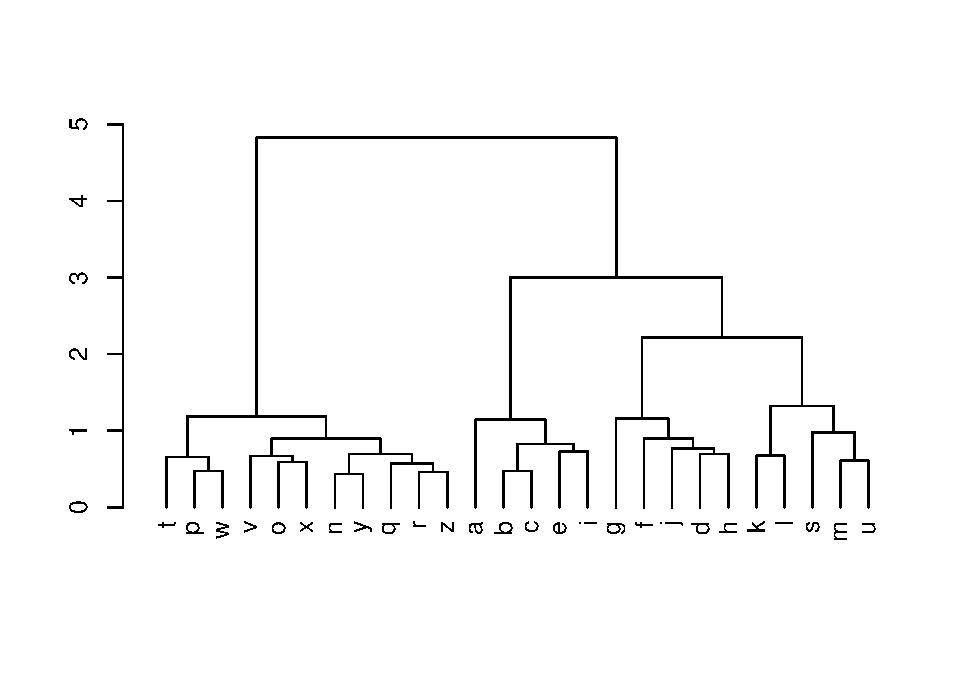
\includegraphics{BF_ms_1_files/figure-latex/Hierarchical clustering sighted-1.pdf}

\begin{verbatim}
##  [1] 20 16 23 22 15 24 14 25 17 18 26  1  2  3  5  9  7  6 10  4  8 11 12 19 13
## [26] 21
\end{verbatim}

\begin{verbatim}
##   average    single  complete      ward 
## 0.3185801 0.1944902 0.4879093 0.6774162
\end{verbatim}

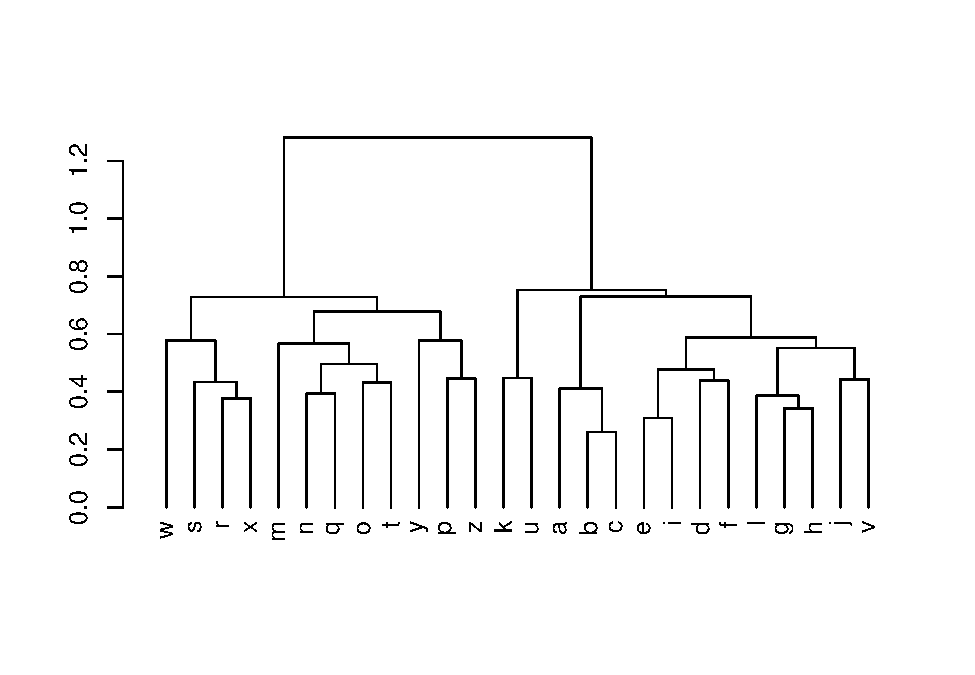
\includegraphics{BF_ms_1_files/figure-latex/Hierarchical clustering sighted-2.pdf} 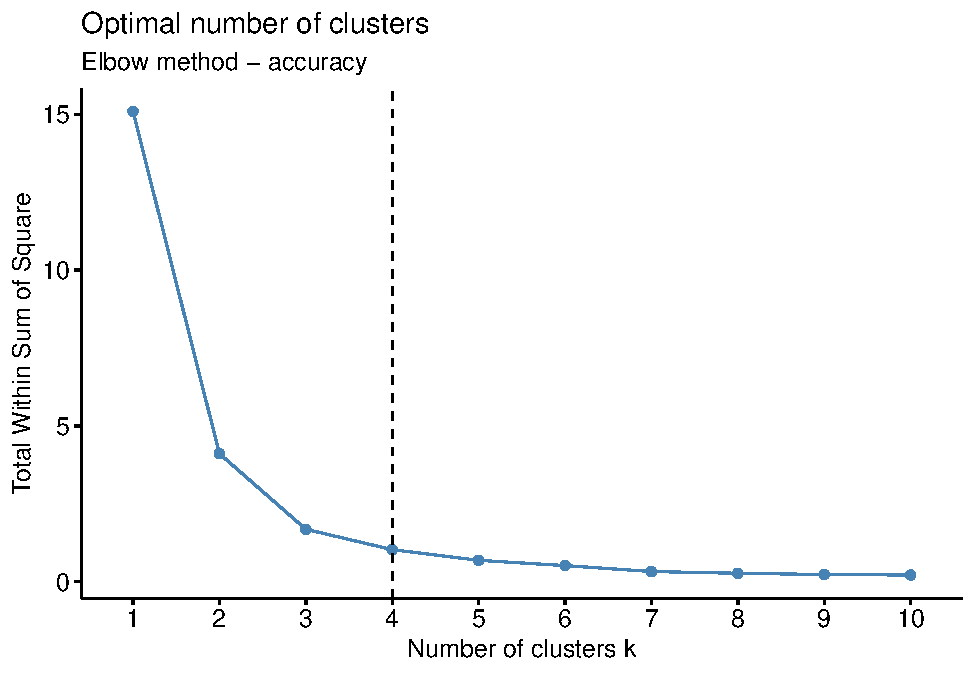
\includegraphics{BF_ms_1_files/figure-latex/Hierarchical clustering sighted-3.pdf} 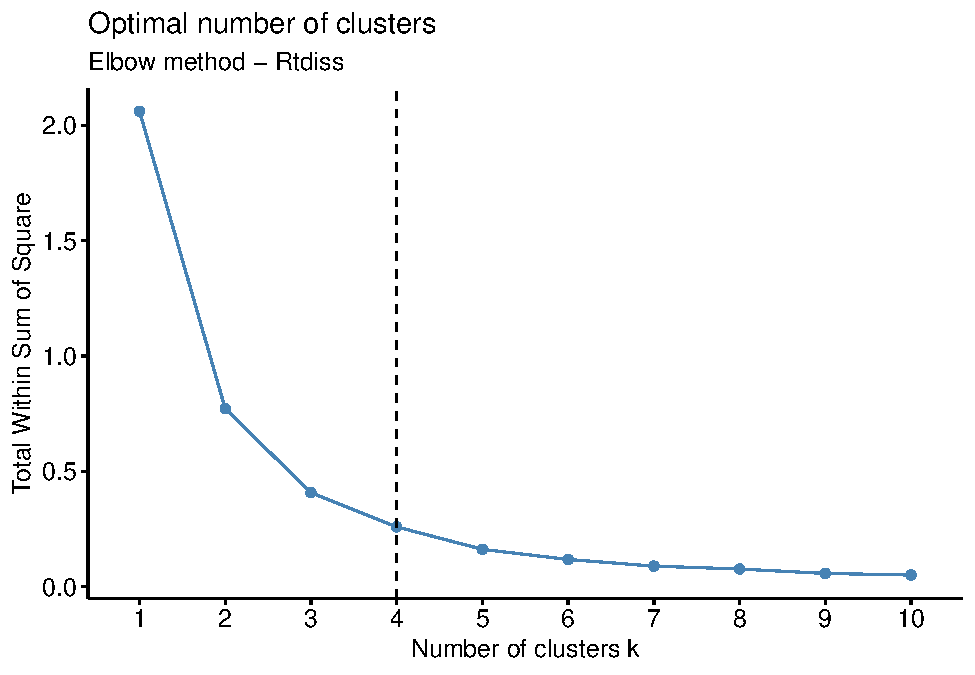
\includegraphics{BF_ms_1_files/figure-latex/Hierarchical clustering sighted-4.pdf}

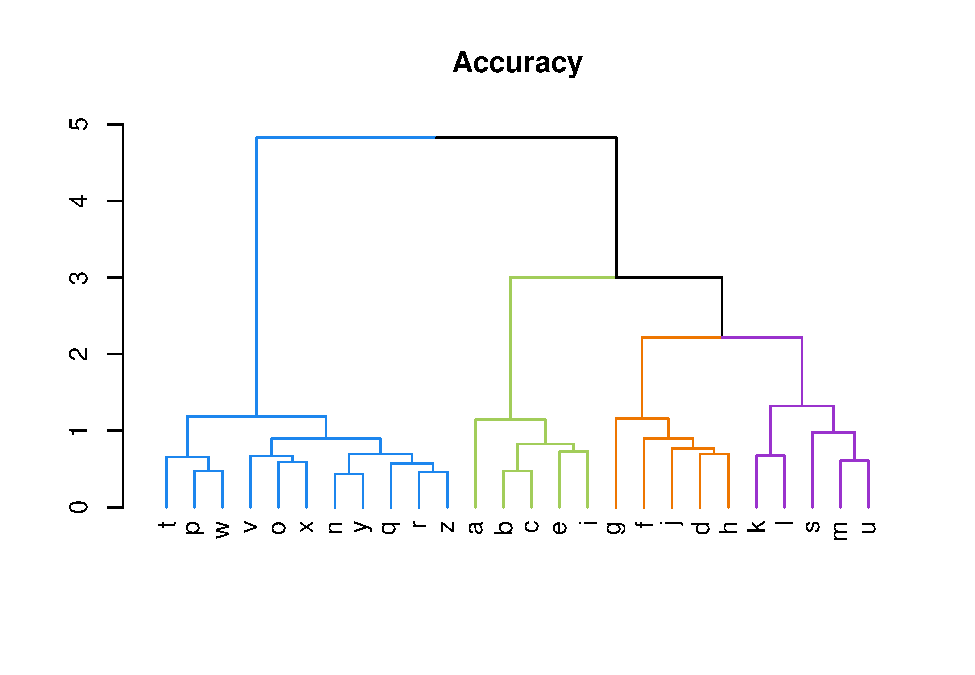
\includegraphics{BF_ms_1_files/figure-latex/Dendrograms with color sighted -1.pdf} 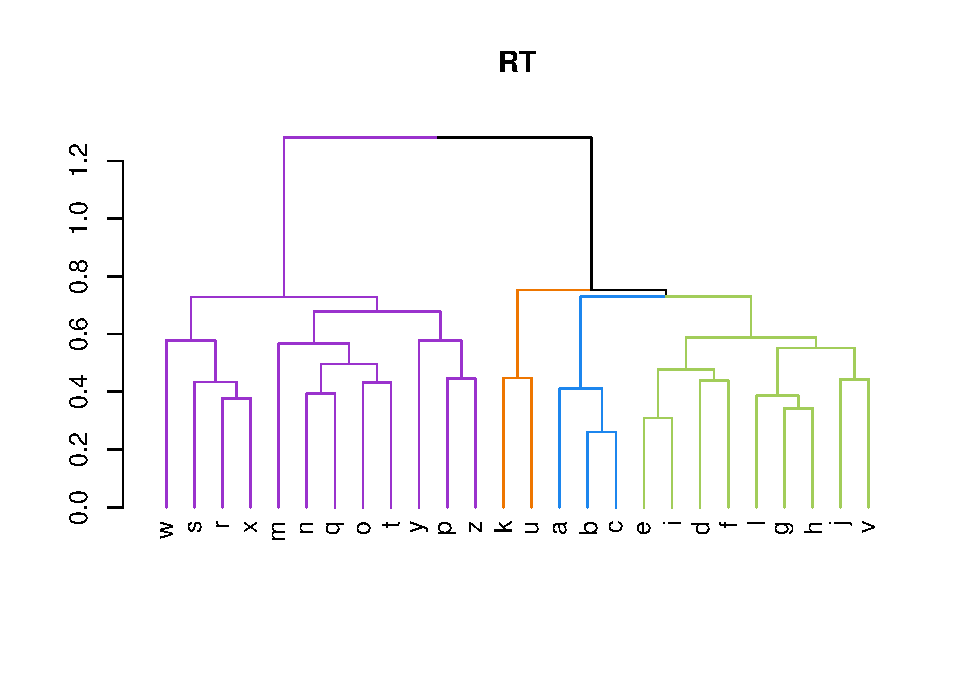
\includegraphics{BF_ms_1_files/figure-latex/Dendrograms with color sighted -2.pdf}

\hypertarget{discussion}{%
\subsection{Discussion}\label{discussion}}

\hypertarget{experiment-2-ciegos}{%
\section{Experiment 2: Ciegos}\label{experiment-2-ciegos}}

\hypertarget{motor-control}{%
\subsubsection{Motor Control}\label{motor-control}}

\begin{itemize}
\tightlist
\item
  file = ``motor\_control\_BF-ino''
\item
  speed = 7000rpm (left to right); 260 rpm (right to left --\textgreater{} because of Miguel)
\item
  distance = 250 steps (\textasciitilde4.5cm)
\end{itemize}

\hypertarget{remember.-to-calculate-speed}{%
\paragraph{REMEMBER. To calculate speed:}\label{remember.-to-calculate-speed}}

\begin{enumerate}
\def\labelenumi{\arabic{enumi}.}
\tightlist
\item
  steps/mm = 200\emph{1/2}20 = 5
\item
  mm/rev = 200/5 = 40 (IN VALENCIA - CHI different because different pulley)
\item
  mm/sec = 40*rpm/60
\end{enumerate}

\hypertarget{method-1}{%
\subsection{Method}\label{method-1}}

\hypertarget{participants-1}{%
\subsubsection{Participants}\label{participants-1}}

24 blind adult individuals\ldots{}

\hypertarget{material}{%
\subsubsection{Material}\label{material}}

All combinations. 5 lists (some 4\ldots{} PANDEMIC)

\hypertarget{procedure-1}{%
\subsubsection{Procedure}\label{procedure-1}}

\hypertarget{data-analysis-1}{%
\subsubsection{Data analysis}\label{data-analysis-1}}

\hypertarget{results-1}{%
\subsection{Results}\label{results-1}}

\begin{verbatim}
## 
##  Paired t-test
## 
## data:  Acc.orders$MAcc1 and Acc.orders$MAcc2
## t = 0.67851, df = 324, p-value = 0.4979
## alternative hypothesis: true difference in means is not equal to 0
## 95 percent confidence interval:
##  -0.003492687  0.007170277
## sample estimates:
## mean of the differences 
##             0.001838795
\end{verbatim}

\begin{verbatim}
## 
##  Paired t-test
## 
## data:  RT.orders.blind$MNRT1 and RT.orders.blind$MNRT2
## t = -1.6644, df = 324, p-value = 0.09701
## alternative hypothesis: true difference in means is not equal to 0
## 95 percent confidence interval:
##  -0.01314649  0.00109665
## sample estimates:
## mean of the differences 
##            -0.006024921
\end{verbatim}

\begin{tabular}{l|r|r|r|r|r|r|r|r|r|r|r|r|r|r|r|r|r|r|r|r|r|r|r|r|r|r}
\hline
  & a & b & c & d & e & f & g & h & i & j & k & l & m & n & o & p & q & r & s & t & u & v & w & x & y & z\\
\hline
a & NA & 0.948 & 1.099 & 0.970 & 0.954 & 1.045 & 0.996 & 0.962 & 1.037 & 0.956 & 1.000 & 1.016 & 0.993 & 0.964 & 0.966 & 0.946 & 1.000 & 0.943 & 0.984 & 1.010 & 0.992 & 0.952 & 0.968 & 0.945 & 1.070 & 0.948\\
\hline
b & 0.948 & NA & 1.022 & 1.006 & 0.992 & 1.022 & 1.005 & 1.020 & 1.002 & 1.004 & 0.950 & 1.045 & 0.923 & 1.001 & 0.980 & 0.996 & 0.970 & 1.000 & 1.001 & 0.988 & 0.931 & 0.955 & 0.970 & 0.970 & 0.970 & 0.976\\
\hline
c & 1.099 & 1.022 & NA & 1.028 & 0.946 & 0.960 & 0.957 & 0.965 & 0.966 & 0.986 & 0.977 & 0.960 & 0.942 & 0.959 & 0.945 & 0.954 & 1.022 & 0.985 & 0.931 & 0.967 & 0.977 & 0.975 & 0.978 & 0.945 & 0.914 & 0.962\\
\hline
d & 0.970 & 1.006 & 1.028 & NA & 1.129 & 1.100 & 0.990 & 1.018 & 0.986 & 1.047 & 1.035 & 1.003 & 0.972 & 0.967 & 0.957 & 0.958 & 0.945 & 0.985 & 0.967 & 0.998 & 0.924 & 0.972 & 1.000 & 0.994 & 0.986 & 0.964\\
\hline
e & 0.954 & 0.992 & 0.946 & 1.129 & NA & 0.988 & 1.139 & 1.011 & 1.056 & 0.994 & 0.963 & 0.944 & 0.966 & 0.948 & 1.027 & 0.931 & 0.980 & 0.996 & 0.970 & 0.962 & 0.942 & 0.933 & 1.027 & 0.968 & 0.909 & 0.979\\
\hline
f & 1.045 & 1.022 & 0.960 & 1.100 & 0.988 & NA & 1.085 & 1.064 & 0.995 & 1.086 & 1.006 & 1.008 & 0.951 & 0.997 & 0.955 & 0.943 & 1.085 & 1.007 & 1.072 & 0.969 & 0.979 & 0.954 & 0.994 & 0.967 & 0.980 & 0.980\\
\hline
g & 0.996 & 1.005 & 0.957 & 0.990 & 1.139 & 1.085 & NA & 1.061 & 0.974 & 1.011 & 0.926 & 1.012 & 0.974 & 0.966 & 0.992 & 1.044 & 1.089 & 1.030 & 0.976 & 0.994 & 0.978 & 0.962 & 0.968 & 0.973 & 1.084 & 0.990\\
\hline
h & 0.962 & 1.020 & 0.965 & 1.018 & 1.011 & 1.064 & 1.061 & NA & 0.999 & 1.130 & 0.946 & 0.992 & 0.941 & 0.999 & 0.988 & 0.990 & 0.960 & 1.010 & 1.009 & 0.982 & 0.959 & 0.997 & 1.041 & 0.990 & 0.963 & 1.004\\
\hline
i & 1.037 & 1.002 & 0.966 & 0.986 & 1.056 & 0.995 & 0.974 & 0.999 & NA & 1.107 & 1.008 & 0.946 & 0.992 & 0.954 & 0.974 & 1.006 & 0.951 & 0.984 & 1.034 & 0.980 & 0.951 & 0.944 & 0.960 & 0.972 & 0.967 & 0.999\\
\hline
j & 0.956 & 1.004 & 0.986 & 1.047 & 0.994 & 1.086 & 1.011 & 1.130 & 1.107 & NA & 0.936 & 0.976 & 0.906 & 1.010 & 0.983 & 0.918 & 0.972 & 0.993 & 0.992 & 0.978 & 0.977 & 0.983 & 1.007 & 0.958 & 0.973 & 0.968\\
\hline
k & 1.000 & 0.950 & 0.977 & 1.035 & 0.963 & 1.006 & 0.926 & 0.946 & 1.008 & 0.936 & NA & 0.980 & 1.060 & 1.039 & 1.030 & 1.002 & 0.955 & 1.010 & 0.990 & 0.960 & 1.229 & 0.978 & 1.038 & 1.000 & 0.994 & 0.990\\
\hline
l & 1.016 & 1.045 & 0.960 & 1.003 & 0.944 & 1.008 & 1.012 & 0.992 & 0.946 & 0.976 & 0.980 & NA & 1.006 & 0.950 & 0.966 & 1.056 & 0.980 & 1.064 & 0.976 & 0.996 & 1.030 & 1.015 & 0.998 & 0.996 & 0.993 & 0.980\\
\hline
m & 0.993 & 0.923 & 0.942 & 0.972 & 0.966 & 0.951 & 0.974 & 0.941 & 0.992 & 0.906 & 1.060 & 1.006 & NA & 0.994 & 0.999 & 0.993 & 0.974 & 0.988 & 0.991 & 0.992 & 1.095 & 0.967 & 0.972 & 1.070 & 1.031 & 0.964\\
\hline
n & 0.964 & 1.001 & 0.959 & 0.967 & 0.948 & 0.997 & 0.966 & 0.999 & 0.954 & 1.010 & 1.039 & 0.950 & 0.994 & NA & 1.173 & 1.046 & 1.020 & 1.038 & 1.002 & 1.082 & 1.034 & 0.988 & 1.018 & 1.036 & 1.069 & 1.151\\
\hline
o & 0.966 & 0.980 & 0.945 & 0.957 & 1.027 & 0.955 & 0.992 & 0.988 & 0.974 & 0.983 & 1.030 & 0.966 & 0.999 & 1.173 & NA & 0.990 & 1.036 & 1.014 & 0.986 & 0.982 & 1.009 & 0.971 & 1.060 & 1.030 & 1.059 & 1.287\\
\hline
p & 0.946 & 0.996 & 0.954 & 0.958 & 0.931 & 0.943 & 1.044 & 0.990 & 1.006 & 0.918 & 1.002 & 1.056 & 0.993 & 1.046 & 0.990 & NA & 1.140 & 1.023 & 1.042 & 1.076 & 0.949 & 1.068 & 1.023 & 1.039 & 1.012 & 0.992\\
\hline
q & 1.000 & 0.970 & 1.022 & 0.945 & 0.980 & 1.085 & 1.089 & 0.960 & 0.951 & 0.972 & 0.955 & 0.980 & 0.974 & 1.020 & 1.036 & 1.140 & NA & 1.152 & 1.064 & 1.054 & 0.973 & 0.982 & 1.076 & 1.029 & 1.028 & 1.044\\
\hline
r & 0.943 & 1.000 & 0.985 & 0.985 & 0.996 & 1.007 & 1.030 & 1.010 & 0.984 & 0.993 & 1.010 & 1.064 & 0.988 & 1.038 & 1.014 & 1.023 & 1.152 & NA & 0.983 & 1.075 & 0.985 & 1.102 & 1.179 & 0.956 & 1.036 & 1.047\\
\hline
s & 0.984 & 1.001 & 0.931 & 0.967 & 0.970 & 1.072 & 0.976 & 1.009 & 1.034 & 0.992 & 0.990 & 0.976 & 0.991 & 1.002 & 0.986 & 1.042 & 1.064 & 0.983 & NA & 1.116 & 1.006 & 0.968 & 1.062 & 0.953 & 0.982 & 0.966\\
\hline
t & 1.010 & 0.988 & 0.967 & 0.998 & 0.962 & 0.969 & 0.994 & 0.982 & 0.980 & 0.978 & 0.960 & 0.996 & 0.992 & 1.082 & 0.982 & 1.076 & 1.054 & 1.075 & 1.116 & NA & 1.018 & 1.020 & 1.047 & 0.955 & 0.996 & 0.974\\
\hline
u & 0.992 & 0.931 & 0.977 & 0.924 & 0.942 & 0.979 & 0.978 & 0.959 & 0.951 & 0.977 & 1.229 & 1.030 & 1.095 & 1.034 & 1.009 & 0.949 & 0.973 & 0.985 & 1.006 & 1.018 & NA & 1.050 & 0.996 & 1.146 & 0.977 & 1.006\\
\hline
v & 0.952 & 0.955 & 0.975 & 0.972 & 0.933 & 0.954 & 0.962 & 0.997 & 0.944 & 0.983 & 0.978 & 1.015 & 0.967 & 0.988 & 0.971 & 1.068 & 0.982 & 1.102 & 0.968 & 1.020 & 1.050 & NA & 1.050 & 1.008 & 1.023 & 1.002\\
\hline
w & 0.968 & 0.970 & 0.978 & 1.000 & 1.027 & 0.994 & 0.968 & 1.041 & 0.960 & 1.007 & 1.038 & 0.998 & 0.972 & 1.018 & 1.060 & 1.023 & 1.076 & 1.179 & 1.062 & 1.047 & 0.996 & 1.050 & NA & 0.985 & 1.056 & 1.095\\
\hline
x & 0.945 & 0.970 & 0.945 & 0.994 & 0.968 & 0.967 & 0.973 & 0.990 & 0.972 & 0.958 & 1.000 & 0.996 & 1.070 & 1.036 & 1.030 & 1.039 & 1.029 & 0.956 & 0.953 & 0.955 & 1.146 & 1.008 & 0.985 & NA & 1.109 & 1.088\\
\hline
y & 1.070 & 0.970 & 0.914 & 0.986 & 0.909 & 0.980 & 1.084 & 0.963 & 0.967 & 0.973 & 0.994 & 0.993 & 1.031 & 1.069 & 1.059 & 1.012 & 1.028 & 1.036 & 0.982 & 0.996 & 0.977 & 1.023 & 1.056 & 1.109 & NA & 1.115\\
\hline
z & 0.948 & 0.976 & 0.962 & 0.964 & 0.979 & 0.980 & 0.990 & 1.004 & 0.999 & 0.968 & 0.990 & 0.980 & 0.964 & 1.151 & 1.287 & 0.992 & 1.044 & 1.047 & 0.966 & 0.974 & 1.006 & 1.002 & 1.095 & 1.088 & 1.115 & NA\\
\hline
\end{tabular}

\begin{tabular}{l|r|r|r|r|r|r|r|r|r|r|r|r|r|r|r|r|r|r|r|r|r|r|r|r|r|r}
\hline
  & a & b & c & d & e & f & g & h & i & j & k & l & m & n & o & p & q & r & s & t & u & v & w & x & y & z\\
\hline
a & NA & 1.055 & 0.910 & 1.031 & 1.049 & 0.957 & 1.004 & 1.040 & 0.964 & 1.047 & 1.000 & 0.984 & 1.007 & 1.038 & 1.035 & 1.057 & 1.000 & 1.061 & 1.017 & 0.991 & 1.008 & 1.050 & 1.033 & 1.058 & 0.934 & 1.055\\
\hline
b & 1.055 & NA & 0.978 & 0.994 & 1.008 & 0.979 & 0.995 & 0.980 & 0.998 & 0.997 & 1.053 & 0.957 & 1.083 & 1.000 & 1.020 & 1.004 & 1.030 & 1.000 & 0.999 & 1.012 & 1.074 & 1.047 & 1.031 & 1.031 & 1.031 & 1.025\\
\hline
c & 0.910 & 0.978 & NA & 0.972 & 1.057 & 1.041 & 1.045 & 1.036 & 1.035 & 1.015 & 1.024 & 1.042 & 1.062 & 1.043 & 1.058 & 1.049 & 0.978 & 1.015 & 1.075 & 1.034 & 1.024 & 1.026 & 1.022 & 1.059 & 1.094 & 1.040\\
\hline
d & 1.031 & 0.994 & 0.972 & NA & 0.886 & 0.909 & 1.010 & 0.982 & 1.015 & 0.955 & 0.966 & 0.997 & 1.029 & 1.034 & 1.045 & 1.044 & 1.059 & 1.015 & 1.034 & 1.002 & 1.082 & 1.029 & 1.000 & 1.006 & 1.014 & 1.037\\
\hline
e & 1.049 & 1.008 & 1.057 & 0.886 & NA & 1.012 & 0.878 & 0.989 & 0.947 & 1.006 & 1.038 & 1.059 & 1.035 & 1.055 & 0.973 & 1.074 & 1.020 & 1.004 & 1.031 & 1.040 & 1.062 & 1.072 & 0.973 & 1.033 & 1.100 & 1.021\\
\hline
f & 0.957 & 0.979 & 1.041 & 0.909 & 1.012 & NA & 0.922 & 0.939 & 1.005 & 0.921 & 0.994 & 0.992 & 1.052 & 1.003 & 1.047 & 1.061 & 0.921 & 0.993 & 0.932 & 1.032 & 1.021 & 1.048 & 1.006 & 1.034 & 1.020 & 1.020\\
\hline
g & 1.004 & 0.995 & 1.045 & 1.010 & 0.878 & 0.922 & NA & 0.943 & 1.027 & 0.989 & 1.080 & 0.988 & 1.026 & 1.035 & 1.008 & 0.958 & 0.918 & 0.971 & 1.025 & 1.006 & 1.022 & 1.039 & 1.033 & 1.028 & 0.922 & 1.010\\
\hline
h & 1.040 & 0.980 & 1.036 & 0.982 & 0.989 & 0.939 & 0.943 & NA & 1.001 & 0.885 & 1.058 & 1.008 & 1.063 & 1.001 & 1.012 & 1.011 & 1.042 & 0.991 & 0.991 & 1.018 & 1.043 & 1.003 & 0.961 & 1.011 & 1.038 & 0.997\\
\hline
i & 0.964 & 0.998 & 1.035 & 1.015 & 0.947 & 1.005 & 1.027 & 1.001 & NA & 0.903 & 0.992 & 1.058 & 1.008 & 1.049 & 1.027 & 0.994 & 1.052 & 1.016 & 0.967 & 1.020 & 1.052 & 1.059 & 1.042 & 1.029 & 1.034 & 1.001\\
\hline
j & 1.047 & 0.997 & 1.015 & 0.955 & 1.006 & 0.921 & 0.989 & 0.885 & 0.903 & NA & 1.068 & 1.025 & 1.104 & 0.991 & 1.017 & 1.089 & 1.028 & 1.007 & 1.008 & 1.023 & 1.024 & 1.017 & 0.993 & 1.044 & 1.027 & 1.033\\
\hline
k & 1.000 & 1.053 & 1.024 & 0.966 & 1.038 & 0.994 & 1.080 & 1.058 & 0.992 & 1.068 & NA & 1.020 & 0.943 & 0.962 & 0.971 & 0.999 & 1.047 & 0.990 & 1.011 & 1.042 & 0.813 & 1.022 & 0.963 & 1.000 & 1.006 & 1.011\\
\hline
l & 0.984 & 0.957 & 1.042 & 0.997 & 1.059 & 0.992 & 0.988 & 1.008 & 1.058 & 1.025 & 1.020 & NA & 0.994 & 1.053 & 1.035 & 0.947 & 1.020 & 0.940 & 1.025 & 1.004 & 0.970 & 0.985 & 1.002 & 1.004 & 1.007 & 1.020\\
\hline
m & 1.007 & 1.083 & 1.062 & 1.029 & 1.035 & 1.052 & 1.026 & 1.063 & 1.008 & 1.104 & 0.943 & 0.994 & NA & 1.006 & 1.001 & 1.007 & 1.026 & 1.013 & 1.009 & 1.009 & 0.913 & 1.034 & 1.029 & 0.934 & 0.969 & 1.037\\
\hline
n & 1.038 & 1.000 & 1.043 & 1.034 & 1.055 & 1.003 & 1.035 & 1.001 & 1.049 & 0.991 & 0.962 & 1.053 & 1.006 & NA & 0.853 & 0.956 & 0.980 & 0.963 & 0.998 & 0.924 & 0.967 & 1.013 & 0.982 & 0.965 & 0.935 & 0.869\\
\hline
o & 1.035 & 1.020 & 1.058 & 1.045 & 0.973 & 1.047 & 1.008 & 1.012 & 1.027 & 1.017 & 0.971 & 1.035 & 1.001 & 0.853 & NA & 1.011 & 0.965 & 0.986 & 1.015 & 1.018 & 0.991 & 1.030 & 0.943 & 0.971 & 0.944 & 0.777\\
\hline
p & 1.057 & 1.004 & 1.049 & 1.044 & 1.074 & 1.061 & 0.958 & 1.011 & 0.994 & 1.089 & 0.999 & 0.947 & 1.007 & 0.956 & 1.011 & NA & 0.878 & 0.977 & 0.960 & 0.929 & 1.054 & 0.936 & 0.978 & 0.962 & 0.988 & 1.008\\
\hline
q & 1.000 & 1.030 & 0.978 & 1.059 & 1.020 & 0.921 & 0.918 & 1.042 & 1.052 & 1.028 & 1.047 & 1.020 & 1.026 & 0.980 & 0.965 & 0.878 & NA & 0.868 & 0.939 & 0.948 & 1.027 & 1.018 & 0.929 & 0.972 & 0.973 & 0.958\\
\hline
r & 1.061 & 1.000 & 1.015 & 1.015 & 1.004 & 0.993 & 0.971 & 0.991 & 1.016 & 1.007 & 0.990 & 0.940 & 1.013 & 0.963 & 0.986 & 0.977 & 0.868 & NA & 1.017 & 0.930 & 1.015 & 0.907 & 0.849 & 1.047 & 0.965 & 0.955\\
\hline
s & 1.017 & 0.999 & 1.075 & 1.034 & 1.031 & 0.932 & 1.025 & 0.991 & 0.967 & 1.008 & 1.011 & 1.025 & 1.009 & 0.998 & 1.015 & 0.960 & 0.939 & 1.017 & NA & 0.896 & 0.995 & 1.034 & 0.941 & 1.049 & 1.018 & 1.035\\
\hline
t & 0.991 & 1.012 & 1.034 & 1.002 & 1.040 & 1.032 & 1.006 & 1.018 & 1.020 & 1.023 & 1.042 & 1.004 & 1.009 & 0.924 & 1.018 & 0.929 & 0.948 & 0.930 & 0.896 & NA & 0.982 & 0.980 & 0.955 & 1.048 & 1.004 & 1.026\\
\hline
u & 1.008 & 1.074 & 1.024 & 1.082 & 1.062 & 1.021 & 1.022 & 1.043 & 1.052 & 1.024 & 0.813 & 0.970 & 0.913 & 0.967 & 0.991 & 1.054 & 1.027 & 1.015 & 0.995 & 0.982 & NA & 0.952 & 1.004 & 0.873 & 1.024 & 0.995\\
\hline
v & 1.050 & 1.047 & 1.026 & 1.029 & 1.072 & 1.048 & 1.039 & 1.003 & 1.059 & 1.017 & 1.022 & 0.985 & 1.034 & 1.013 & 1.030 & 0.936 & 1.018 & 0.907 & 1.034 & 0.980 & 0.952 & NA & 0.952 & 0.993 & 0.978 & 0.998\\
\hline
w & 1.033 & 1.031 & 1.022 & 1.000 & 0.973 & 1.006 & 1.033 & 0.961 & 1.042 & 0.993 & 0.963 & 1.002 & 1.029 & 0.982 & 0.943 & 0.978 & 0.929 & 0.849 & 0.941 & 0.955 & 1.004 & 0.952 & NA & 1.015 & 0.947 & 0.913\\
\hline
x & 1.058 & 1.031 & 1.059 & 1.006 & 1.033 & 1.034 & 1.028 & 1.011 & 1.029 & 1.044 & 1.000 & 1.004 & 0.934 & 0.965 & 0.971 & 0.962 & 0.972 & 1.047 & 1.049 & 1.048 & 0.873 & 0.993 & 1.015 & NA & 0.902 & 0.919\\
\hline
y & 0.934 & 1.031 & 1.094 & 1.014 & 1.100 & 1.020 & 0.922 & 1.038 & 1.034 & 1.027 & 1.006 & 1.007 & 0.969 & 0.935 & 0.944 & 0.988 & 0.973 & 0.965 & 1.018 & 1.004 & 1.024 & 0.978 & 0.947 & 0.902 & NA & 0.897\\
\hline
z & 1.055 & 1.025 & 1.040 & 1.037 & 1.021 & 1.020 & 1.010 & 0.997 & 1.001 & 1.033 & 1.011 & 1.020 & 1.037 & 0.869 & 0.777 & 1.008 & 0.958 & 0.955 & 1.035 & 1.026 & 0.995 & 0.998 & 0.913 & 0.919 & 0.897 & NA\\
\hline
\end{tabular}

\begin{verbatim}
##   average    single  complete      ward 
## 0.6361242 0.5132008 0.7165643 0.8340732
\end{verbatim}

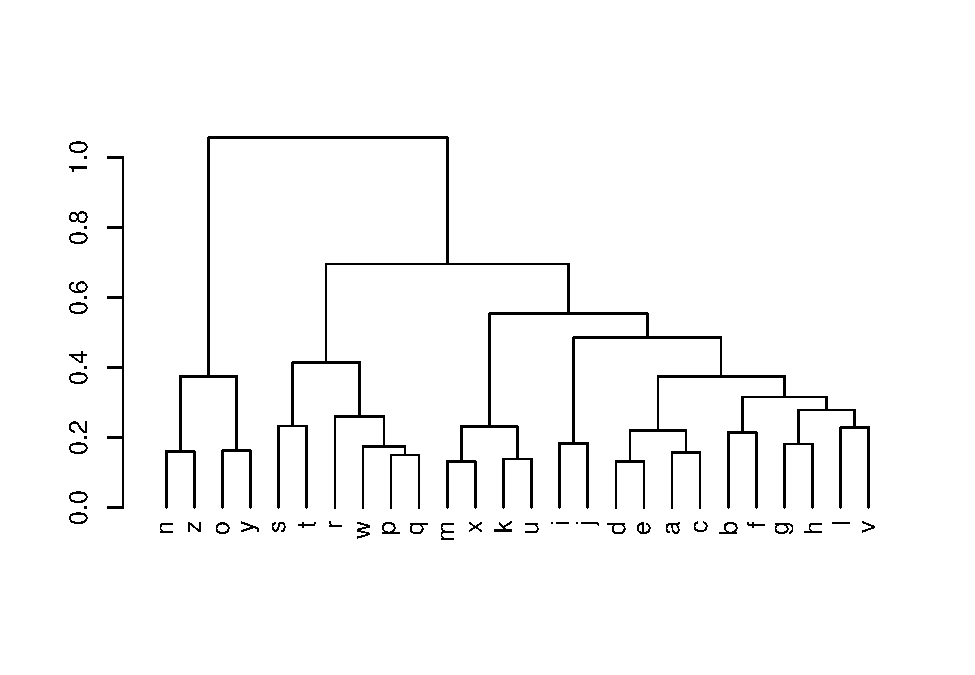
\includegraphics{BF_ms_1_files/figure-latex/Hierarchical clustering bl-1.pdf}

\begin{verbatim}
##  [1] 14 26 15 25 19 20 18 23 16 17 13 24 11 21  9 10  4  5  1  3  2  6  7  8 12
## [26] 22
\end{verbatim}

\begin{verbatim}
##   average    single  complete      ward 
## 0.4173949 0.2259740 0.5526253 0.7378997
\end{verbatim}

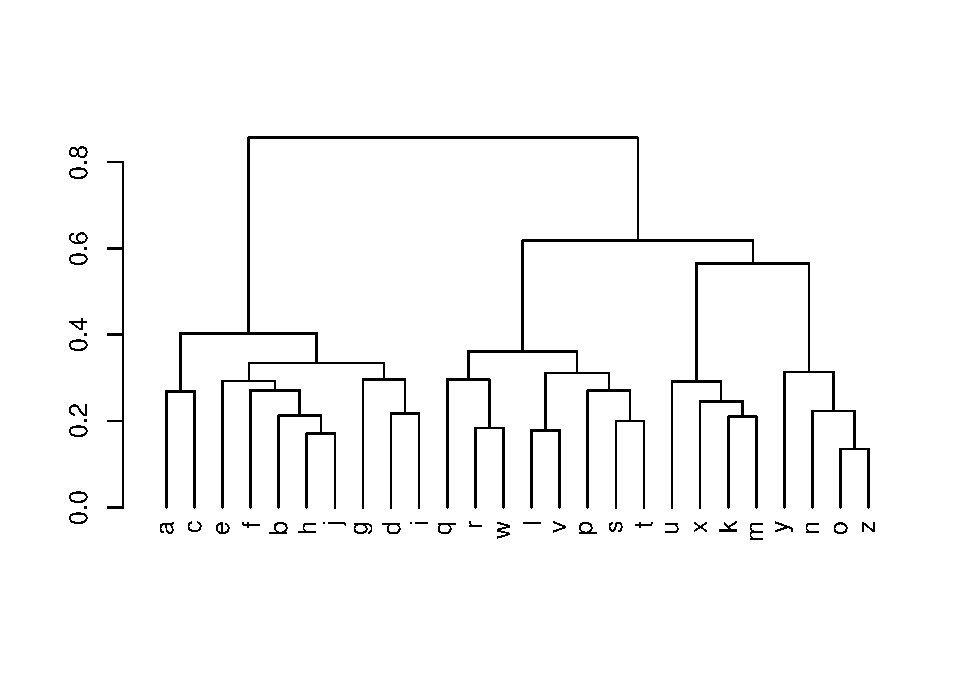
\includegraphics{BF_ms_1_files/figure-latex/Hierarchical clustering bl-2.pdf} 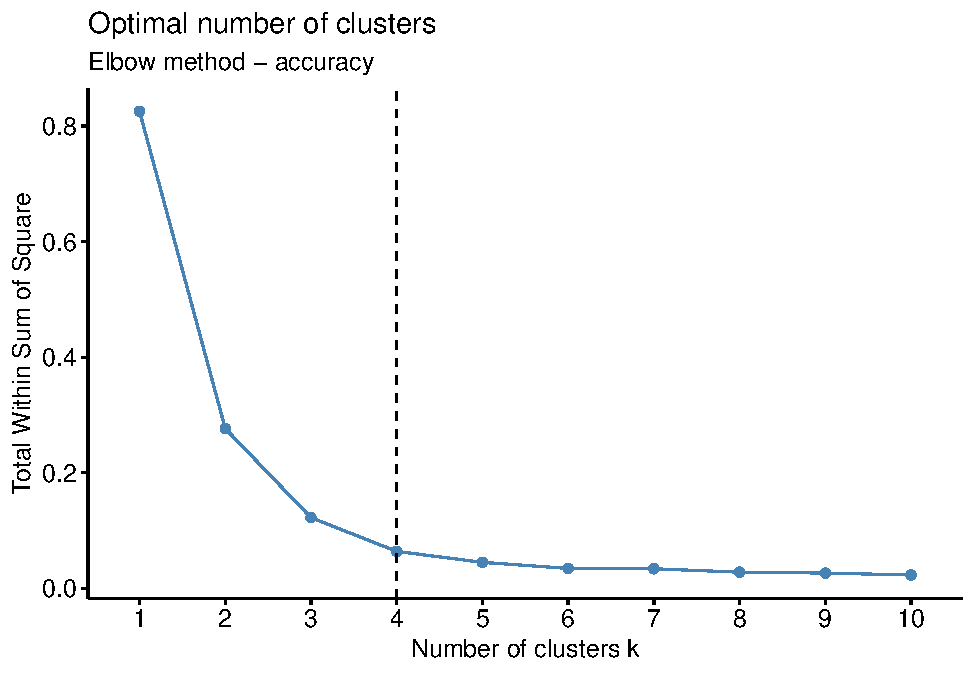
\includegraphics{BF_ms_1_files/figure-latex/Hierarchical clustering bl-3.pdf} 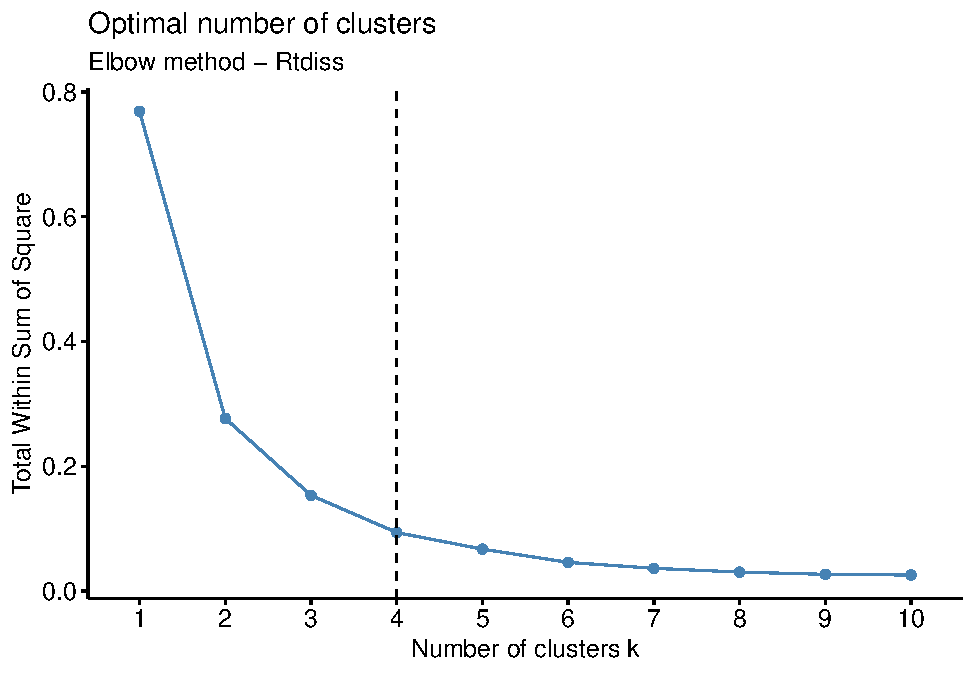
\includegraphics{BF_ms_1_files/figure-latex/Hierarchical clustering bl-4.pdf}

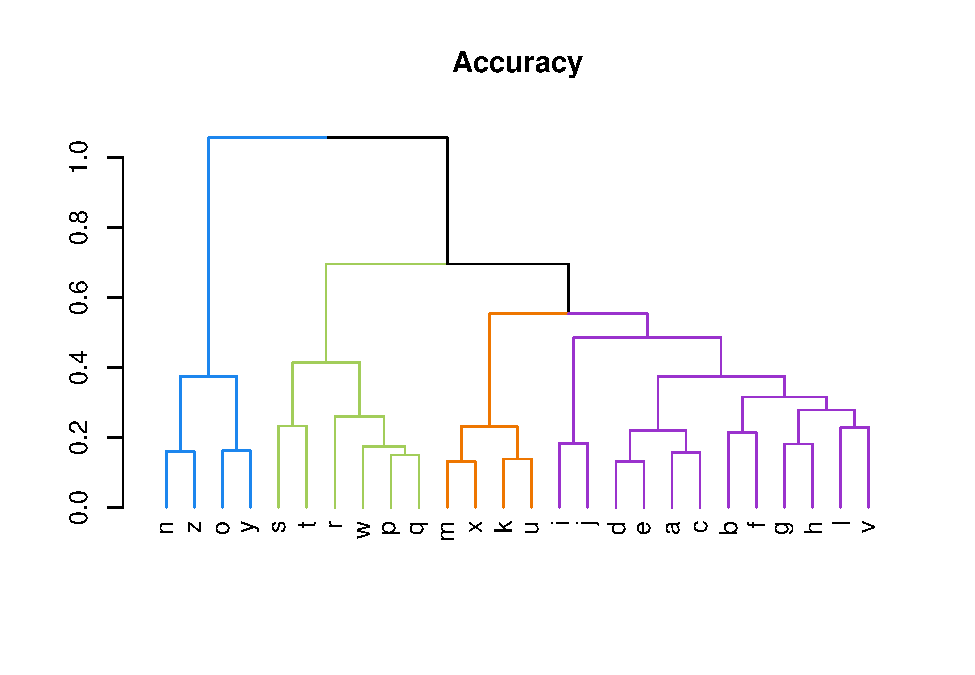
\includegraphics{BF_ms_1_files/figure-latex/Dendrograms with color bl-1.pdf} 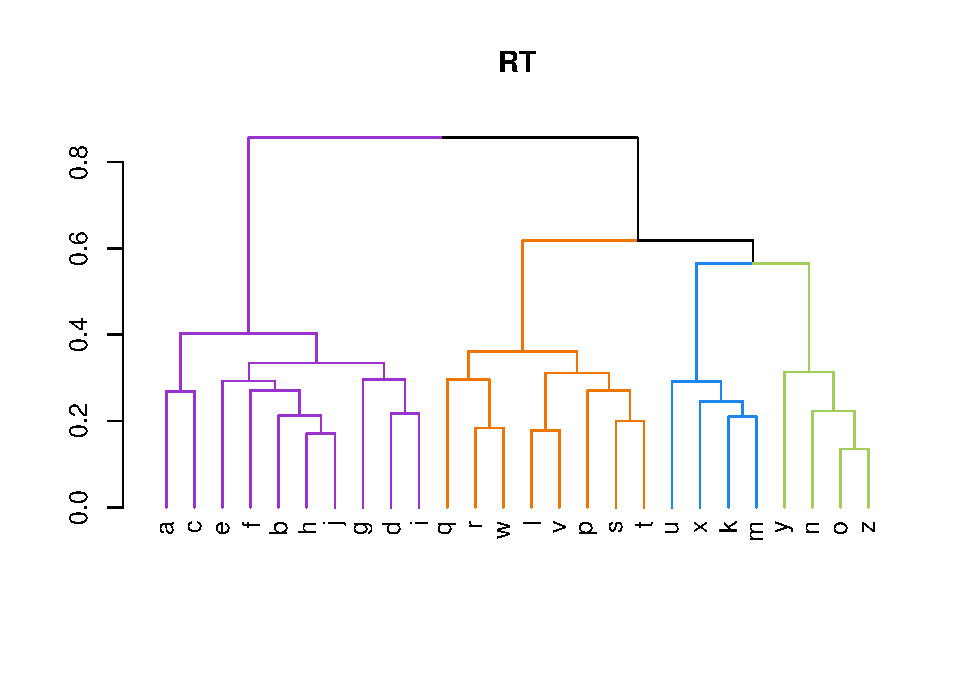
\includegraphics{BF_ms_1_files/figure-latex/Dendrograms with color bl-2.pdf}

\hypertarget{discussion-1}{%
\subsection{Discussion}\label{discussion-1}}

\hypertarget{general-discussion}{%
\section{General Discussion}\label{general-discussion}}

\newpage

\hypertarget{references}{%
\section{References}\label{references}}

\begingroup
\setlength{\parindent}{-0.5in}
\setlength{\leftskip}{0.5in}

\hypertarget{refs}{}
\begin{CSLReferences}{0}{0}
\end{CSLReferences}

\endgroup


\end{document}
